\section{Modelling}

\subsection{Mathematical Formulation}

The model propsed by Anderson et al.~\cite{anderson_continuous_1998,anderson_mathematical_2000} and Chaplain et al.~\cite{anderson_continuous_1998,chaplain_mathematical_2006-1,franssen_mathematical_2019}, extended with terms for modelling cell proliferation and extracellular matrix renewal consists of a system of coupled partial differential equations with zero-flux boundry conditions: 
\begin{align}
	\frac{\partial c}{\partial t} &= D_c \Delta c - \chi \nabla (c\nabla e)  + \mu_1 c\left(1-\frac{c}{c_0}-\frac{e}{e_0}\right)\label{eq1}\\
	\frac{\partial e}{\partial t} &= -\delta m e  + \mu_2 c\left(1-\frac{c}{c_0}-\frac{e}{e_0}\right)\label{eq2}\\
	\frac{\partial m}{\partial t} &= D_m \Delta c + \mu_3 c - \lambda m\label{eq3}
\end{align}
\begin{align}
	c (-D_c \nabla c + c \chi\nabla e) &= 0 \label{eq4}\\
	c (-D_m\nabla m ) &= 0\label{eq5}
\end{align}

with the free parameters $D_c$, $D_m$, $\chi$, $\delta$, $\mu_1$, $\mu_2$, $\mu_3$ and $\lambda$. \newline
The variable $c$ describes the tumor cell density, $e$ the concentration of the extracellular matrix and $m$ the matrix-degrading enzyme concentration. All of those functions are mathematically defined to be mapping a 1,2 or 3 dimensional spacial value $x$ and a temporal value $t$ to a scalar value describing the respective quantity at a specific point in space and time $(x,t)$, $\{c,e,m\} : \mathbb{R}^{3} \times \mathbb{R} \rightarrow \mathbb{R}$.\newline
To derive the expression of the tumor cell density $c$ we are going to assume that the tumor cell's movement is subject to two influences, haptotaxis and random movement. Haptotaxis is a directed migratory response of cells to gradients of fixed or bound chemicals~\cite{anderson_continuous_1998} and random movement is influenced by for example mechanical stress, electric charge or other such physical effects~\cite{Merino-Casallo2022-di}. To get an expression for how much or how fast the tumor cells move, we need to define what flux is. Flux is defined to be the amount of a substance  which crosses a unit area in unit time. Incorporating the two assumed influencing factors into our mathematical model we define the haptotatic flux $J_{hapto}$ and random flux $J_{random}$:
\begin{align*}
    J_{hapto} = \chi c \nabla e \\
    J_{random} = -D_c \nabla c
\end{align*}
$\chi$ is the haptotactic flux coefficient and $D_c$ is a random mobility coefficient. In general these Parameters could also be a function of both extracellular matrix and matrix-degrading enzyme concentration. Knowing that cells grow over time and proliferate, we want to respect this in our model with a term for tumor cell proliferation: $\mu_1 c (1-\frac{c}{c_0} - \frac{e}{e_0})$.\newline  
The idea is that this term describes the cell proliferation with a logisitic growth model respecting spacial limiting factors of already present extracellular matrix molecules and tumour cells, $\mu_1$ describes the rate at which proliferation happens. In the initial model proposed by Anderson et al.~\cite{anderson_continuous_1998, anderson_mathematical_2000} and Chaplain et al.~\cite{anderson_continuous_1998,chaplain_mathematical_2006,chaplain_mathematical_2006-1,franssen_mathematical_2019}, they did not respect proliferation of tumor cells and extracellular matrix renewal and applied a conservation equation for the tumor cells which yields:
\begin{align*}
    \frac{\partial c}{\partial t} = -\nabla (J_{hapto} + J_{random}) \\
    \frac{\partial c}{\partial t} = -\nabla (\chi c \nabla e -D_c \nabla c ) \\
    \frac{\partial c}{\partial t} = D_c \Delta c - \chi \nabla (c\nabla e)
\end{align*}
The extended model incorporates proliferation and renewal into this conservation formula resulting in equation~\ref{eq1}:
\begin{align*}
    \frac{\partial c}{\partial t} = -\nabla (J_{hapto} + J_{random}) + \mu_1 c (1-\frac{c}{c_0} - \frac{e}{e_0}) \\
    \frac{\partial c}{\partial t} = D_c \Delta c - \chi \nabla (c\nabla e) + \mu_1 c (1-\frac{c}{c_0} - \frac{e}{e_0})
\end{align*}
To model the extracellular-matrix concentration $e$, we assume that the enzymes degrade the extracellular matrix upon contact. This assumption is simply modeled by the equation:
\begin{align*}
    \frac{\partial e}{\partial t} = -\delta m e
\end{align*}
where $\delta$ is a positive constant describing this degradation process. For the extended model we add a term describing the renewal process of the extracellular matrix: 
\begin{align*}
    \frac{\partial e}{\partial t} = -\delta m e + \mu_2 c (1 - \frac{c}{c_0} - \frac{e}{e_0})
\end{align*}
with $mu_2$ being the coefficient describing the rate of the renewal process.\newline
Modelling the matrix-degrading enzyme concentration $m$, we combine a diffusion term with production and decay terms. The diffusion term is described like in tumor cell concentration, with the addition that haptotatic fluxes are neglected and only random mobility is assumed, $J_{random} = -D_m \nabla m$. The production term depends on the tumor cell density $c$ and the decay term on the extracellular matrix concentration $m$. Incorporating this gives us equation~\ref{eq3}:
\begin{align*}
    \frac{\partial m}{\partial t} = \nabla J_{random} + \mu c - \lambda e \\
    \frac{\partial m}{\partial t} = D_m \Delta m + \mu_3 c - \lambda m
\end{align*}
$\mu_3$ and $\delta$ describing production and decay coefficients .


\subsection{Numerical Formulation and Parameters}

To make solving the model easier we are first going to non-dimensionalise all the equations~\ref{eq1} to~\ref{eq5} in a standard way, with the goal to rescale the space domain to a unit size domain $\Omega$. For one space dimension this results in the unit interval $[0,1]$, for two the unit square $[0,1] \times [0,1]$ and for three spacial dimensions the unit cube $[0,1] \times [0,1] \times [0,1]$. \newline
We start with non-dimensionalising the three continuous variables $c,e,m$:
\begin{align*}
    \tilde{c} = \frac{c}{c_0} \\
    \tilde{e} = \frac{e}{e_0} \\
    \tilde{m} = \frac{m}{m_0}  
\end{align*}
Next we rescale distance with an appropriate length scale $L$ (e.g. the maximum invasion distance of the cancer at this early stage of invasion $0.1-1cm$) and time with $\tau = \frac{L^2}{D}$ ($D$ being a chemical diffusion coefficient $D\approx 10^{-6} \frac{cm^2}{s}$)~\cite{anderson_mathematical_2000}. \newline
Modifying the system's free parameters $D_c, \chi, \delta, D_m, \mu_3, \lambda$ gives us:  
\begin{center}
    $d_c = \frac{D_c}{D},\quad \gamma = \chi \frac{e_0}{D},\quad \eta = \tau m_0 \delta,\quad d_m = \frac{D_m}{D},\quad \alpha = \tau \mu_3 \frac{c_0}{m_0},\quad \beta = \tau \lambda$.
\end{center} 
with $D$ being the aforementioned reference chemical diffusion coefficient.\newline 
These modifications make the new system of coupled partial differential equations, where the tildes are dropped and we assume $t$ as $\tau$ for simplicities' sake, with also updated zero-flux boundary conditions:
\begin{align}
	\frac{\partial c}{\partial t} &= d_c \Delta c - \gamma \nabla (c\nabla e)  + \mu_1 c\left(1-\frac{c}{c_0}-\frac{e}{e_0}\right)\label{eq:6}\\
	\frac{\partial e}{\partial t} &= -\eta m e  + \mu_2 e\left(1-\frac{c}{c_0}-\frac{e}{e_0}\right)\label{eq:7}\\
	\frac{\partial m}{\partial t} &= d_m \Delta c + \alpha c - \beta m\label{eq:8}
\end{align}
\begin{align}
	\zeta (-d_c \nabla c + c \gamma \nabla e) &= 0\label{eq:9}\\
	\zeta (-d_m\nabla m ) &= 0\label{eq:10}
\end{align}
where $\zeta$ is an outward unit normal vector.\newline 
In order to use the Finite Element Method we will change to the variational formulation. If we assume each species to be in the Hilbert space $H^1(\Omega)$, the variational formulation can be derived by multiplying with a test function $\varphi_i$, integrating over the domain $\Omega$ and use integration by parts and the Gauss theorem. This will give us a broader solution space and reduces the requirements of the solution regarding differentiability. With $\left(\cdot, \cdot\right)$ denoting the $L^2$-scalar product on $\Omega$ the following equation system results:
\begin{align}
    \left(\frac{\partial c}{\partial t}, \varphi_c\right) &=
        - d_c\left(\nabla c, \nabla \varphi_c\right) + \gamma \left(c\nabla e, \nabla \varphi_c\right) + \mu_1 \left(c \left(1-\frac{c}{c_0} - \frac{e}{e_0}\right), \varphi_c\right) \label{eq:11}\\
    \left(\frac{\partial e}{\partial t}, \varphi_e\right) &=  -\eta \left( me, \varphi_e\right) + \mu_2 \left(e\left(1-\frac{c}{c_0}-\frac{e}{e_0}\right),\varphi_e\right) \label{eq:12}\\
    \left(\frac{\partial m}{\partial t}, \varphi_m\right) &= -d_m \left(\nabla m,\nabla \varphi_m\right) + \alpha \left(c,\varphi_m\right) - \beta \left(m,\varphi_m\right) \label{eq:13}
\end{align}

\begin{figure}[h]
    \centering
    \label{fig:Initial_Value_Distribution}
    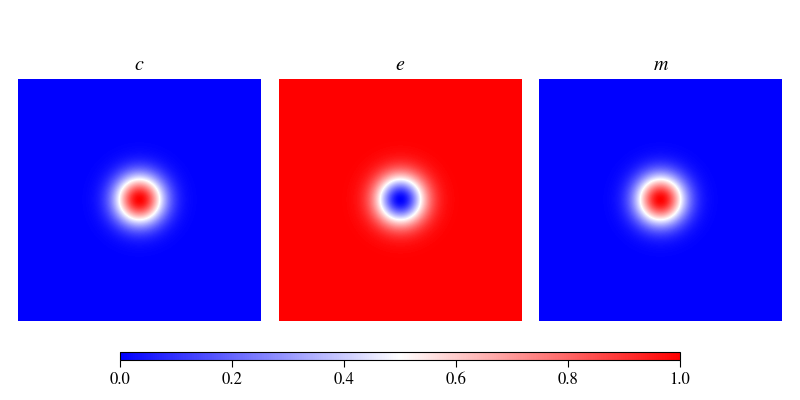
\includegraphics[width=0.8\textwidth]{resources/images/2D_initial_conditions_homogenous_ECM.png}
    \caption{Visualization of the initial value distribution for an experiment in two space dimensions with a homogenous extracellular matrix}
    \label{fig:2D_homogenous_ECM_initial}
\end{figure}
Non-dimensionalising our system of equations allows us to formulate the initial conditions in simple terms. Since our aim is to describe both homogenous as well as heterogenous extracellular matrix structures we have to respect this in regard to the initial conditions for the variable $e$.\newline 
Assuming that at dimensionless time $t=0$ there is already a nodule of cells located at the center of the unit domain $\Omega$ we define the initial conditions for the tumour cell denisity as:
\begin{align*}
    c(x,0)= \exp(\frac{-(x-0.5)^2}{\epsilon})
\end{align*}
where for our experiments we used the value $\epsilon=0.01$.\newline
Assuming that these tumour cells have already produced an amount of matrix-degrading enzymes, we can define the inital conditions for the variable $m$ the same way as the tumour cells were:
\begin{align*}
    m(x,0) = 0.5 c(x,0) = 0.5 \exp(\frac{-(x-mean)^2}{\epsilon})
\end{align*}
Considering the initial strucutre of the extracellular matrix we suppose that the tumour cells have already degraded some of the extracellular matrix, especially at the center where the tumour cells are located. Furthermore we have to differentiate now between homogenous and heterogenous extracellular matrix structure. If the ECM has a homogenous structure, which means that it is evenly distributed in space we set its initial value as:
\begin{align*}
    e(x,0) = 1 - 0.5 c(x,0)
\end{align*}
Figure~\ref{fig:2D_homogenous_ECM_initial} shows a 2D plot of the initial conditions using the homogenous extracellular matrix structure.\newline 
\begin{figure}[h]
    \centering
    \label{fig:Initial_Value_Distribution}
    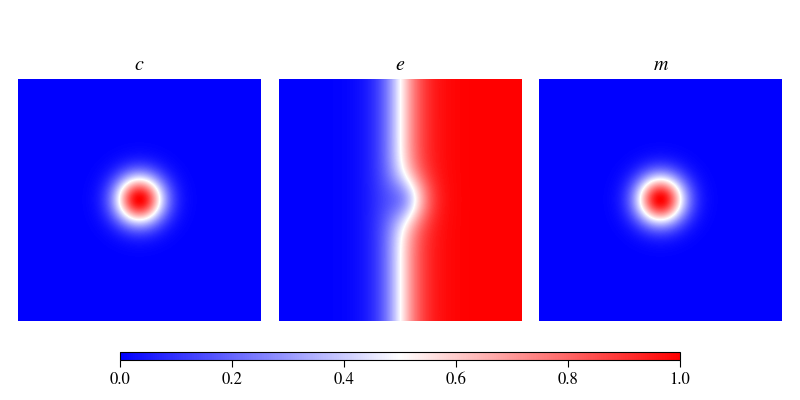
\includegraphics[width=0.8\textwidth]{resources/images/2D_initial_conditions_heterogenous_ECM.png}
    \caption{Visualization of the initial value distribution for an experiment in two space dimensions with a heterogenous extracellular matrix}
    \label{fig:2D_heterogenous_ECM_initial}
\end{figure}
When we now assume a heterogenous ECM strucuture the initial conditions change to:
\begin{align*}
    e(x,0) = 1 - 0.5 c(x,0)
\end{align*}
In figure~\ref{fig:2D_heterogenous_ECM_initial} these change of structure is clearly shown in the middle plot, where red inidcates that only on the left side there are extracellular matrix molecules.